\chapter{Background}\label{ch:background}

To establish a clear foundation for the concepts and definitions introduced throughout this thesis, a fundamental overview of the key topics relevant to this research will be provided. This includes an introduction to \ac{RTS}, \acf{IPC}, and synchronisation techniques, with a particular focus on wait-free synchronisation. Additionally, the Rust programming language will be examined, as it serves as the primary development environment for this study. Furthermore, existing synchronisation methods in \ac{RTS} will be explored to contextualise the motivation and contributions of this work.

\section{Real-Time Systems}\label{sec:real-time}

In \ac{RTS}, the correctness of the system depends not only depend on the logical results of computations, but also on timing constraints. These systems can be classified into \ac{HRTS} or \ac{SRTS}. \ac{HRTS} have strict timing constraints, and missing a constraint is considered a system failure. The system must guarantee that every timing constraint has to be met. A use case would be industrial automation where all the machines and robotic modules must communicate with each other as quickly as possible to ensure the manufacturing line is not blocked. \cite{HardSoftRealTime}

On the other hand, \ac{SRTS} try to stick to the timing constraints as much as possible, but missing some timing constraints is not considered a system failure. In terms of infrastructure, \ac{SRTS} are similar to \ac{HRTS}, since it is still considered important to meet these timing constraints. An example would be a multimedia system where it would be considered fine if sometimes frames are dropped to guarantee the video stream. \cite{HardSoftRealTime}

Sometimes these two systems appear in combination, where some functions have hard real-time constraints and some have soft real-time constraints. Krishna et al. gives a good example in his paper where he describes that for the Apollo 11 mission some components for the landing processes had soft real-time behaviour and the rest still functioned with hard real-time constraints. \cite{HardSoftRealTime}

Since the work field of this thesis is within \ac{HRTS}, the term \ac{RTS} will be used synonymously with the terminology \ac{HRTS}.

\section{\acf{IPC}}\label{sec:ipc}

Processes used in a \ac{RTS} also have to share information with each other so the system can function. So some kind of \ac{IPC} is needed. \ac{IPC} allows processes to share information with each other using different kinds of methods like a shared memory region, which is the method used and explained later in this thesis \cite{IPCMechanisms}. In general, \ac{IPC} is needed in all computing systems, because processes often need to work together (e.g. a producer process passes data to a consumer process) \cite{IPCMechanisms}. Let's take the brake-by-wire technology as an example. Brake-by-wire is a technology for driverless cars where some mechanical and hydraulic components from the braking systems are replaced by wires to transmit braking signals, since there is no longer a driver to press the brake pedal \cite{BrakeByWire}. This of course requires different processes to share information. In the context of this thesis this kind of communication requires strict timing constraints as stated before, since any kind of blockage in a brake-by-wire systrem could lead to a catastrophe.

\subsection{Shared Memory}\label{subsec:shared-memory}

To achieve any kind of information sharing between processes, these processes will need to have access to the same data regularly. With a shared memory segment, multiple processes can have access to the same memory location. So all processes which are part of the \ac{IPC} can read and write to this common memory space avoiding unnecessary data copies. With that, processes exchange information by directly manipulating memory. This kind of \ac{IPC} is particularly useful for real-time applications, which handle large volumes of data or are required to quickly transfer data between sensors and control tasks. It is also important to note that the section of code that manages these data accesses by different processes is called the critical section. The problem with this is that the system somehow has to manage how the processes access the shared memory segment. This is mostly done by using different kinds of synchronisation techniques. Without any synchronisation mechanism race conditions or inconsistent data can occur. \cite{sharedmem}

\section{Synchronisation}\label{sec:synchronization}

Synchronisation is important for \ac{IPC} in \ac{RTS}, especially when processes communicate via shared memory. Communication through shared memory always has a risk of race conditions and data inconsistency if the processes are not properly synchronised. Traditional synchronisation techniques ensure mutual exclusion (only one process at a time uses shared resource) thus avoiding race conditions and ensuring data consistency. Race conditions happen when for example two processes write to the same resource. Let's take a single counter instance with value 17 as a shared resource in a shared memory region. If one process p1 and one process p2 increments that number, the end result should be 19. But what could happen is that p1 could read the value 17 before p2 increments it and then before p1 increments that value p2 could also read the value 17. Now internally both processes increment that number to 18 and both processes would write 18 to that shared resource. To understand this example in more detail \cref{fig:race-condition} visualises a race condition with threads. 

The difference between processes and threads is just that threads are part of a process which can perform multiple tasks via threads simultaneously within that process. Another difference that will later be important in this thesis is that processes have their own private memory space, while threads share the memory space of the process they are part of. Thus, a process cannot naturally access the memory of another process. The following concept in \cref{fig:race-condition} can still be used for processes. \cite{processesVSthreads}

\begin{figure}[!ht]
    \centering
    \captionsetup{justification=centering}
    \caption{Race condition between two threads, which write to the same shared variable.}
    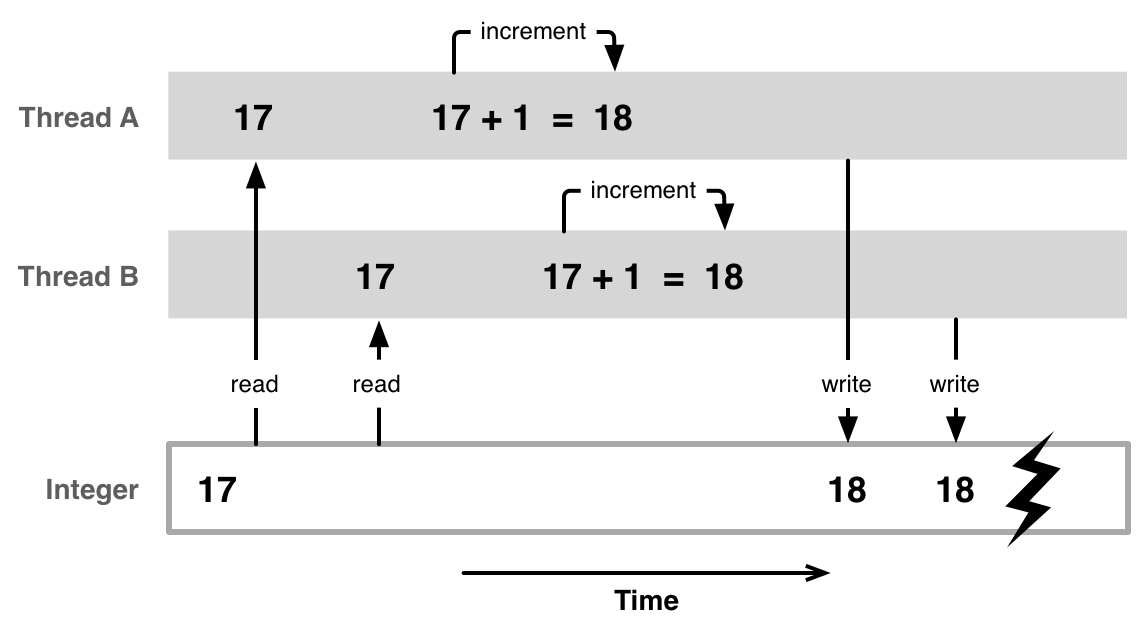
\includegraphics[width=115mm]{images/race-condition.png}
    \cite{Race-Condition}
    \label{fig:race-condition}
\end{figure}

\subsection{Mutual Exclusion}\label{subsec:mutual-exclusion}

As discussed, mutual exclusion does only allow one process or thread to access the shared resource at a time. This includes that if a process p1 already accessed the shared resource x and is still working on it, a second process p2, which tries to access that shared resource x has to wait until the process p1 finishes its task, where it needs that shared resource x. To achieve this, synchronisation techniques based on locks or semaphores are typically used to block the entry of a process to an already accessed and in use shared resource of another process. See \cref{fig:mutual-exclusion} to gain a deeper understanding on how this works. This paper will not go into detail how traditional synchronisation techniques like locks or semaphores work, since for this work it is only important that these kinds of methods manage the access of processes to shared resources in shared memory via some kind of locks. A process will acquire a lock to access a shared resource and will release it when its task is done. Another process trying to access the same resource while it's in use has to wait until the lock is released for that resource.

\begin{figure}[!ht]
    \centering
    \captionsetup{justification=centering}
    \caption{Mutual exclusion between three tasks(processes), which access the same critical section. Multiple processes need to stop working and just wait for other processes to finish their work. See the waiting phase of the processes.}
    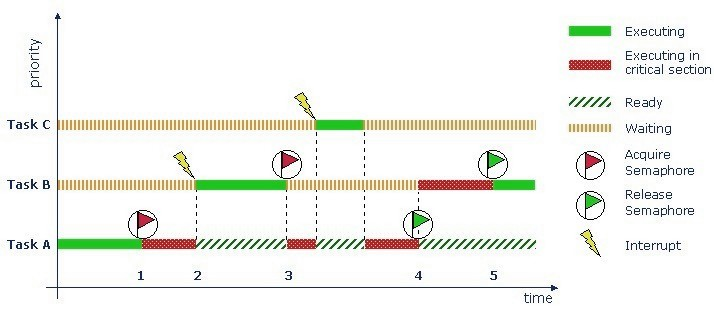
\includegraphics[width=135mm]{images/mutual_exclusion.jpg}
    \cite{MutualExclusion}
    \label{fig:mutual-exclusion}
\end{figure}

Clearly, this approach inherently relies on blocking processes. This may lead to several issues, including deadlocks, process starvation, or priority inversion leading to unpredictable response times not being able to define timing constraints for \ac{RTS} \cite{brandenburg2019multiprocessorrealtimelockingprotocols}. The sequence which process might acquire the lock first to enter the critical section, when multiple processes wait for the access is mostly set by a scheduler \cite{brandenburg2019multiprocessorrealtimelockingprotocols}. Since wait-free methods explained later in \cref{sec:wait-free} are lock-free, a scheduler is not needed and as a result of that scheduling will not be explained more in detail in this work. The problems mentioned above will be discussed in the following subsubsections:

\begin{figure}[!ht]
    \centering
    \captionsetup{justification=centering}
    \caption{Deadlock between two processes, which wait for each other to release the needed resources.}
    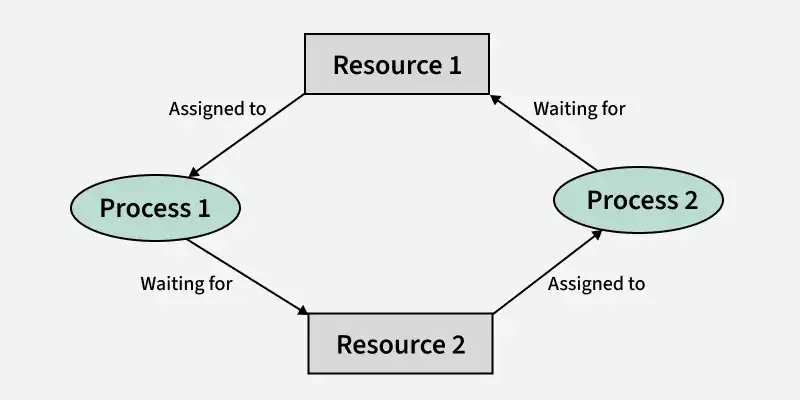
\includegraphics[width=110mm]{images/deadlock.png}
    \cite{Deadlock}
    \label{fig:deadlock}
\end{figure}

\subsubsection{Process Starvation}\label{subsubsec:process-starvation}

What happens when multiple processes try to enter the shared resource one after another, and one process repeatedly fails to acquire a lock to enter the critical section. This one  process would wait for an indefinite time and will never enter the shared resource, which is called as process starvation. This usually happens when a synchronisation method allows one or more processes to make progress while ignoring a particular process or processes. This mostly happens in environments where some sort of process prioritisation exists and processes are classified into low and high priority processes. When there are always a lot of high priority and some low priority processes available, it might happen that these low priority processes will never be able to enter the critical section. This is a problem, since these low priority processes might be important for the system too. \cite{Starvation}

\subsubsection{Deadlock}\label{subsubsec:deadlock}

Even worse, what if two or more processes have already accessed a resource and now each waits for the other to release the lock for the resource each of them acquired to furtther work? This results in a situation seen in \cref{fig:deadlock} where these processes now indefinitely wait for each other and never terminate. Thus, the resources held by these waiting processes are never released and are therefore never available to the other process. As one can see, this brings a system into a state which would make no progress any further and would not respond to any command anymore. \cite{chahar2013deadlock}

For instance, a driverless car with a brake-by-wire system, where processes responsible for braking are in a deadlock, the car could eventually not brake if needed and a fatal car crash would happen. 


\subsubsection{Priority Inversion}\label{subsubsec:priority-inversion}

Now let's say no process starvations or deadlocks happen. What could happen too is that a lower priority process already accessed a shared resource and after that a higher priority process needs to access that specific resource too. If the lower priority process now gets delayed, the higher priority process gets delayed too. This would be called priority inversion now; a low priority process delaying a high priority process. \cite{priorityInversion}

\section{Lock-Free Synchronisation}\label{sec:lock-free}

Because of all the problems traditional synchronisation techniques introduce, synchronisation techniques are required that do not block processes with any kind of locking mechanism. One way could be the implementation of lock-free synchronisation techniques. This would allow multiple processes to access the shared resource concurrently. Lock-free synchronisation ensures that at least one process will complete its task in a finite number of steps. However, some processes may be unable to proceed, because lock-free synchronisation does not guarantee that all processes will complete their operations in a finite number of steps. This means that starvation or even priority inversion is still possible, as some processes, even high priority processes may be indefinitely delayed. There are different kinds of mechanisms to achieve this. One way to accomplish lock-freedom for example is the lock-free technique introduced by Michael and Scott, which is also the basis for some other wait-free algorithms.

\subsection{Michael and Scott's Lock-Free Queue}\label{subsec:michael-scott}

Michael and Scott developed an algorithm seen in \cref{alg:michael-scott} using a linked-list as a shared data structure with an enqueue and a dequeue function to introduce lock-freedom. A linked-list is a list containing nodes containing data and a pointer called next which references the next node in the list, which can only be traversed in a single direction. There is also a pointer called head, which references the beginning node of the list and a pointer called tail, which references the end node of the list. The core concept of the algorithm is the enqueue and dequeue functions beginning at lines 7 and 26 in \cref{alg:michael-scott}, which are used to add and remove nodes to the shared data structure. When a process tries to add a node to the list, it first creates a new node and sets its next pointer to \texttt{NULL}, see line 8 to 10 of the enqueue function. Beginning from line 11 to line 23 following happens: The process first checks if the pointer referencing to the next node after the tail node is \texttt{NULL}, see line 15. If it is \texttt{NULL} it tries to link the new node to the end of the list by using a \ac{CAS} seen in line 16. This operation atomically compares the current value of the tail pointer with the expected value and, if they match, updates the tail pointer to point to the new node. The tail itself would be updated in line 24.  \cite{MichaelScottQueue}

So let's say 2 processes p1 and p2 execute up to line 16 one after the other. What could happen now is that if p1 executes line 16 before p2, p2 will fail the \ac{CAS} from line 16. Now if p1 does not execute further, thus not finalising the enqueue with line 24 and p2 retries the loop until line 15, the condition in line 15 would not be \texttt{TRUE} anymore for p1 and p1 would execute lines 19 and 20 to help p2 to finalise its enqueue so other processes can work further with this algorithm. \cite{MichaelScottQueue}

The dequeue function works analogously, but instead of adding a node to the end of the list it removes a node from the front of the list. And since another process which could not finish its enqueue would cause confusion for other processes in the dequeue function, the process which could not finish its enqueue will also be helped in the dequeue function. \cite{MichaelScottQueue}

Initialisation starts at line 1 in \cref{alg:michael-scott}, which is just used to create dummy nodes when there's no node in the list. This just simplifies the algorithm so that the head and tail pointers are not \texttt{NULL}. It can be observed that this approach does not need any locks explained in \cref{sec:synchronization}. However, this approach has one major problem. If for instance process p1 is trying to enqueue, it can happen that the \ac{CAS} loop might fail indefinitely if for an indefinite time other processes are always executing line 16 immediately before p1 could execute line 16. This means that in very high contention scenarios, a process may be delayed indefinitely and starve out. In an \ac{HRTS}, this could lead to violation of timing constraints, since the process would not finish his task in the defined timing window, which is unacceptable. This is why a slightly different approach which guarantees that every process will complete its operation in a finite number of steps is in need. \cite{MichaelScottQueue}

\begin{algorithm}[!ht]
    \centering
    \captionsetup{justification=centering}
    \caption{Michael and Scott's Lock-Free Queue}
    \label{alg:michael-scott}
    \scriptsize
    \begin{algorithmic}[1]

    \Function{Initialize}{Q : pointer to queue\_t}
        \State node = \textbf{new} node() 
        \Comment{Allocate a dummy node}
        \State node.next.ptr = \texttt{NULL}
        \Comment{Make it the only node in the list}
        \State Q.Head = node 
        \Comment{Both Head and Tail point}
        \State Q.Tail = node 
        \Comment{to this dummy node}
    \EndFunction
    
    \Function{Enqueue}{Q : pointer to queue\_t, value : data\_type}
        \State node = \textbf{new} node() 
        \Comment{Allocate a new node from the free list}
        \State node.value = value
        \Comment{Copy enqueue value into node}
        \State node.next.ptr = \texttt{NULL}
        \Comment{Set next pointer of node to NULL}
    
        \Loop 
        \Comment{Keep trying until Enqueue is done}
            \State tail = Q.Tail
            \Comment{Read Tail (pointer + count) together}
            \State next = tail.ptr.next
            \Comment{Read next ptr + count together}
    
            \If{tail == Q.Tail} 
            \Comment{Are tail \& next consistent?}
                \If{next.ptr == \texttt{NULL}}
                \Comment{Tail is the last node?}
                    \If{$CAS(\&\,tail.ptr.next,\; next,\; \langle node,\; next.count+1\rangle)$}
                        \State \textbf{break}
                        \Comment{Link the new node; Enqueue is done}
                    \EndIf
                \Else 
                \Comment{Tail not pointing to the last node}
                    \State CAS($\&$\,Q.Tail,\; tail,\; $\langle$ next.ptr,\; tail.count+1$\rangle$)
                    \Comment{Move Tail forward (helping another enqueuer)}
                \EndIf
            \EndIf
        \EndLoop
    
        \State 
        $CAS(\&\,Q.Tail,\; tail,\; \langle node,\; tail.count+1\rangle)$
        \Comment{Final attempt to swing Tail to the inserted node}
    
    \EndFunction
    
    \Function{Dequeue}{Q : pointer to queue\_t,\; pvalue : pointer to data\_type}
        \Loop
        \Comment{Keep trying until Dequeue is done}
            \State head = Q.Head
            \State tail = Q.Tail
            \State next = head.ptr.next
            \Comment{Read head->next}
    
            \If{head == Q.Head} 
            \Comment{Still consistent?}
                \If{head.ptr == tail.ptr} 
                \Comment{Empty or Tail behind?}
                    \If{next.ptr == \texttt{NULL}}
                    \Comment{Queue is empty}
                        \State \textbf{return} FALSE
                    \Else
                        \Comment{Tail is behind, help move it}
                        \State 
                        $CAS(\&\,Q.Tail,\; tail,\; \langle next.ptr,\; tail.count+1\rangle$)
                    \EndIf
    
                \Else
                    \Comment{No need to adjust Tail}
                    \State *pvalue = next.ptr.value
                    \Comment{Read value before CAS}
                    \If{$CAS(\&\,Q.Head,\; head,\; \langle next.ptr,\; head.count+1\rangle)$}
                        \State \textbf{break}
                        \Comment{Dequeue is done}
                    \EndIf
                \EndIf
            \EndIf
        \EndLoop
    
        \State \textbf{free}(head.ptr)
        \Comment{Safe to free old dummy node}
        \State \textbf{return} TRUE
    
    \EndFunction
    
    \end{algorithmic}
    \cite{MichaelScottQueue}
\end{algorithm} 

While Michael and Scott's algorithm relies on the \ac{CAS} primitive, other atomic primitives provide alternative approaches that other algorithms shown later in this thesis use. An overview on the atomic primitives that are used in this thesis context is given in the following section.

\subsection{Atomic Primitives}\label{subsec:atomic-primitives}
Atomic primitives are hardware instructions that conduct a set of steps atomically, meaning with no interruption from other processes \cite{Atomics}. This will be important in the algorithms analysed later in this thesis, since these primitives are used to implement wait-free synchronisation. There are different kinds of atomic primitives: 

\subsubsection{\acf{LL/SC}}\label{subsubsec:llsc}
Abbreviation of the instructions \ac{LL} and \ac{SC}, which is an operation available on ARM, MIPS and Alpha architectures usually implied with a \ac{VL} instruction.
\begin{itemize}
    \item \ac{LL}(R) returns value of register r
    \item \enquote{\ac{SC}(R, v) changes the value in register R to v and returns true, if and only if no other process performed a successful SC since the most recent call of LL of the current process. So SC fails if the value of the register has changed since it has been read} \cite{Fuchs2014EvaluationOT}
    \item \enquote{\ac{VL}(R) returns true if no other process performed a successful SC on register R, which allows to test a register value without changing it} \cite{Fuchs2014EvaluationOT}
\end{itemize}
\cite{Fuchs2014EvaluationOT}

\subsubsection{\acf{CAS}}\label{subsubsec:compare-and-swap}
In addition to the explanation in \cref{subsec:michael-scott} \ac{CAS} is an atomic primitive that is supported on \enquote{Intel x386, x64 and most general purpose architectures with operands that are restricted to pointer size} \cite{Fuchs2014EvaluationOT}.
\begin{itemize}
    \item \enquote{\ac{CAS}(R,e,n) returns true and sets the value of R to n if the value in R is e. Otherwise, it returns false.} \cite{Fuchs2014EvaluationOT}
\end{itemize}
The problem with \ac{CAS}, beyond the issue explained earlier, in \cref{subsec:michael-scott} is that it can lead to the ABA problem, which can also occur in wait-free algorithms:
\begin{itemize}
    \item Process 1 reads value A from a shared variable.
    \item Process 2 changes the value to B and then back to A.
    \item Process 1's \ac{CAS} operation succeeds, because it compares the value A it read earlier with the current value A, even though the value was changed in between.
\end{itemize}
This is a fundamental limitation of \ac{CAS}. One solution would be to replace \ac{CAS} with \ac{LL/SC}, but that is not possible on x86 processors. So other solutions are needed that are discussed in \cref{ch:implementation}. \cite{Fuchs2014EvaluationOT}

\subsubsection{\ac{DWCAS}}\label{subsubsec:double-compare-and-swap}
This is a \ac{CAS} on two neighbouring memory locations. \cite{Fuchs2014EvaluationOT}

\subsubsection{\ac{DCAS}}\label{subsubsec:double-with-compare-and-swap}
Sometimes also called \ac{CAS}2, is a \ac{CAS} on two independent memory locations. \cite{Fuchs2014EvaluationOT}

\subsubsection{Swap}\label{subsubsec:swap}
Swap is an atomic read-modify-write operation that unconditionally exchanges a value in memory with a new value and returns the old value. Swap(R, v) atomically stores value v into location R and returns the previous value that was in R. This operation always succeeds. \cite{Mateíspmc}.

\subsubsection{\acf{FAA}}\label{subsubsec:fetch-and-add}
This primitive is used to increment \enquote{the value of a variable by a given offset and [return] the result. This instruction always succeeds.} \cite{Fuchs2014EvaluationOT}

\subsubsection{\ac{FAS}}\label{subsubsec:fetch-and-store}
This atomically stores a value in a variable and returns the previous value. This is similar to \ac{CAS}, but it does not require a comparison and a retry loop. This is faster than \ac{CAS}, if conditions before updating do not need to be checked. \cite{Drescher2015GuardedSections}

\section{Wait-Free Synchronisation}\label{sec:wait-free}

Lock-freedom solves the problem of a system getting into a deadlock. But this is not enough, in a fully automated car for example it is undesirable that any process does not complete its task, since that could mean that some processes that are responsible for braking would not finish their work in a worst case scenario. And such an occasion where the car would need to brake a fatal car crash would be the outcome. Consequently, a solution is necessary where every process finishes their task in a finite number of steps instead of just one process. So something is needed that builds upon such mechanisms and extends them. This is exactly what wait-free synchronisation is. It guarantees that every process will complete its operation in a finite number of steps, regardless of contention. This means that even process starvation is by definition not possible anymore. Also priority inversion is eliminated too, because processes do not have to wait for other processes anymore. This ensures system responsiveness and predictability therefore the ability to define strict timing constraints needed for \ac{HRTS} applications. But even wait-free algorithms introduce one problem. Wait-free algorithms are in most cases slower than their lock-free counterparts in execution. A solution for this will be addressed in \cref{ch:related-work} and analysed more in depth in \cref{ch:choosing-the-optimal-wait-free-data-structure}.

\section{Rust Programming Language}\label{sec:rust}

The question now is which programming language suits best for this kind of algorithms. Since a fast communication between the processes is compulsory to meet all \ac{HRTS} timing constraints, the C programming language would be a good choice. C provides low-hardware control and therefore also allows the implementation of fast low-latency communication. What is also important and necessary for a \ac{RTS} is that C does not have an automatic garbage collector, which gets active and stops all processes from working to clean up allocated but no longer used memory space. Because of that all \ac{RTOS} are written in C. The main problem with C is that it does not provide any kind of memory safety, since C implements memory operations that are prone to buffer overflows or control-flow attacks. In the industry around 70\% of vulnerabilities happen due to memory safety issues. If the real-time application would run on an isolated system with no internet connection, this would not be a problem. But in modern automation, where systems need to be connected to the internet for data exchange, such systems would be prone to security attacks. \ac{RTS} nowadays is an integral part in various connected devices, including critical fields such as health or transportation. Consequently, it is extremely important that the security of such devices is guaranteed. With the Rust programming language the problems of memory safety are gone. The difference to C is that it can be as fast as C with the possibility to support low-level control and high-level programming features, while providing memory safety features. The memory safety aspect is achieved by an ownership concept that controls how memory is handled in programmes. This is strictly checked and therefore the executable programme has guaranteed memory safety. In the model every value has a single owner represented by a variable. The owner is in charge of the lifetime and deallocation of that value. Rust will automatically free the memory associated with that value, when the owner goes out of scope. This behaviour is automatically done by using the memory reference feature provided by Rust. Creating such references is called borrowing. This allows the usage of these values without transferring the ownership. These references have their own lifetime, which can be explicitly defined by the programmer or implicitly inferred by Rust's compiler. This ensures that the references are valid and do not exist longer than needed. Hence this can play a role in lock-freedom, which is needed for wait-free synchronisation, since shared resources can be shared with this ownership concept. Additionally, Rust is a type-safe language, which can be helpful during implementation to avoid bugs and errors. As seen, Rust is a good choice for implementing wait-free synchronisation mechanisms for \ac{IPC} in \ac{RTS}. \cite{xu2023rust, culic2022lowRust}. 

Further mechanisms on how Rust handles different kinds of common memory safety issues are solved will not be discussed in detail, as that would go beyond the scope of this thesis. It is only important to know the basics on how Rust is a type-safe and memory-safe programming language, to understand why Rust is used for this work.